% !TEX root = ../thesis.tex

\chapter{Evaluation} \label{evaluation}
\section{Experiment} \label{sec:experiment}
Lets prepare the experiment to validating a long-term linear prediction model for online store orders. We will use experimentation by these steps:\\
\begin{enumerate}
    \item Define the problem and objectives: Clearly define the problem and objectives that the long-term linear prediction model is intended to solve.
    In this case, the objective is to predict online store orders over a long period of time using a linear model.
    \item Gather data: Collect historical data on online store orders, such as order dates, order amounts, and other relevant variables.
    This data will be used to train and validate the long-term linear prediction model. Our data was collect from online system storePredictor
    which is available on storepredictor.com and data are anonymized and pseudonimized to be used for next calculations.
    \item Prepare the data: Clean and preprocess the data to ensure that it is consistent and suitable for use in the long-term linear prediction model.
    This may involve tasks such as removing duplicates, handling missing values, and transforming variables as needed.
    Preprocessing of our data is described in \ref{subsec:preprocessing}
    \item Develop the long-term linear prediction model: Using the historical data, develop a long-term linear prediction model that can
    forecast online store orders over a specified time period, which is detailed described in \ref{sec:extlonglp} and practically applied in \label{subsec:calculate_models}
    \item Validate the model: Once the model is developed, it needs to be validated to ensure that it is accurate and effective.
    This can be done by comparing the model's predictions with actual online store orders over a specified time period, described in \label{subsec:validatibg_models}
    \item Evaluate the results: Analyze the results of the experiment to determine the accuracy of the long-term linear prediction model.
    This will involve calculating metrics such as the mean square error (MSE), r-squared ($R^2$) and the root mean square error (RMSE) \ref{subsec:experimentResults}.
    \item During solving previous steps the model was redefined and revalidate when the results are not satisfactory, refine the model and repeat the validation
    process until an accurate and effective long-term linear prediction model is developed.
\end{enumerate}
In summary, to prepare an experiment to validate a long-term linear prediction model for online store orders, you need to
define the problem and objectives, gather and prepare the data, develop the model, validate it, evaluate the results, and refine and revalidate
the model if necessary.
    \subsection{Preprocessing of input data} \label{subsec:preprocessing}
    Preprocessing the data is an important step in preparing the data for a linear order prediction model. Here are some common
    steps to preprocess the data for linear order prediction:

    \begin{enumerate}
        \item Data cleaning: Remove any irrelevant data or duplicate records in the dataset. In our purpose is to clean the unsuccessfull orders,
        returned orders and fraud orders from competitors to detect power of the store.
        \item Handling missing data: for fill in any missing values in the dataset machine learning algorithms K-Nearest Neighbors (KNN) \ref{sec:knn} will be used
        to check the dataset.
        \item Feature selection: Select the relevant features (predictors) that are likely to have a strong influence on the order
        prediction. This may include variables such as customer demographics, purchase history, product attributes, and marketing campaigns.
        \item Feature scaling: Scale the features so that they are on the same scale to ensure that each feature has equal importance.
        This can be done using normalization or standardization techniques.
        \item Handling categorical variables: Convert categorical variables into numerical values using techniques
        such as one-hot encoding, ordinal encoding, or label encoding.
        \item Dimensionality reduction: If the dataset contains many features, use dimensionality reduction
        techniques such as principal component analysis (PCA) or linear discriminant analysis (LDA) to reduce the number of features and simplify the model.
        \item Handling outliers: Detect and handle any outliers in the dataset using appropriate techniques
        such as Z-score, Tukey’s method, or machine learning algorithms such as Isolation Forest or Local Outlier Factor.
    \end{enumerate}
    Overall, the goal of this steps for linear order prediction experiment is to ensure that the data is clean, complete, and properly
    formatted for use in the linear prediction model. This helps to improve the accuracy and effectiveness of the model in predicting online store orders.
    \subsection{Model for sales forecasting} \label{subsec:calculate_models}
    Let's prepare 4 models to test our theory and result expectation.  Set up MATLAB live script to prepare our dataset, calculate statistical variables and
    develop several versions of linear predictors to get reults of our experiment. We will use this models:
    \begin{enumerate}
        \item Short-term linear prediction 
        Based on linear prediction \ref{subsec:shortlp} we calculate optimal coeficients by \ref{subsec:levinson} and made prediction over our dataset.
        This model is described in equation \ref{eq:slp}.

        \item Extended short-term linear prediction 
        This model is based on linear prediction \ref{subsec:shortlp} with optimal parameters by levinson schema \ref{subsec:levinson}.
        To compare our developed model \label{subsec:extlonglp} and we will prepare similar principle as in equation \ref{eq:eltlp} to the short-term linear
        prediction with results:
        
        \begin{equation} \label{eq:slp}
            \begin{aligned}
                &\hat{y} = \sum_{j=1}^{n} a(j)*y(n-j) * \gamma(t)
            \end{aligned}
        \end{equation}
        \begin{itemize}
            \item $\hat{y}$ is the value of the predicted order
            \item $a(1), a(2), ..., a(n)$ are the prediction coefficients
            \item $y(n-1), y(n-2), ..., y[n-j]$ are the past values of the signal that are used to make the prediction
        \end{itemize}

        \item Long-term linear prediction 
        To compare more linear prediction and check theorem about application of long-term prediction on sales data we will prepare the model
        based on \label{subsec:longlp} and use the equation \ref{eq:ltlp}.

        \item Extended long-term linear prediction
        The last model in our comparison will be our developed model which is based on long-term linear prediction describe in \ref{subsec:longlp} and
        use weights coefficients \ref{sec:weights} to get better results in economics data. This model is describe in equation \ref{eq:eltlp}.
    \end{enumerate}
    % reference to equations: eq:eltlp, 
    All the models will be used dataset prepared in \ref{subsec:preprocessing} and results of prediction is described in \ref{subsec:experimentResults}.
    \subsection{Results} \label{subsec:experimentResults}
        The metrics described in \ref{subsec:comparison} are commonly used to evaluate
        the performance of each prepared models.
        \subsubsection{Short-term linear prediction} \label{subsec:res_slp}
        From our experiment we get R-squared (R²) value of 0.8872 which means that
        88.7\% of the variation in the dependent variable can be explained
        by the independent variables in the model.\\
        In our case, an RMSE of 40.6215 means that on average, the predicted values
        from the model are about 40.6 units away from the actual values.
        And the MSE of 1650.1 means that on average, the squared difference between the
        predicted and actual values is 1650,1.\\
        On figure \ref{fig:slpres} we can see predicted orders and on figure \ref{fig:slpmse}
        is the prediction error. 
        \begin{figure}[h]
            \centering
            \begin{minipage}{0.45\textwidth}
                \centering
                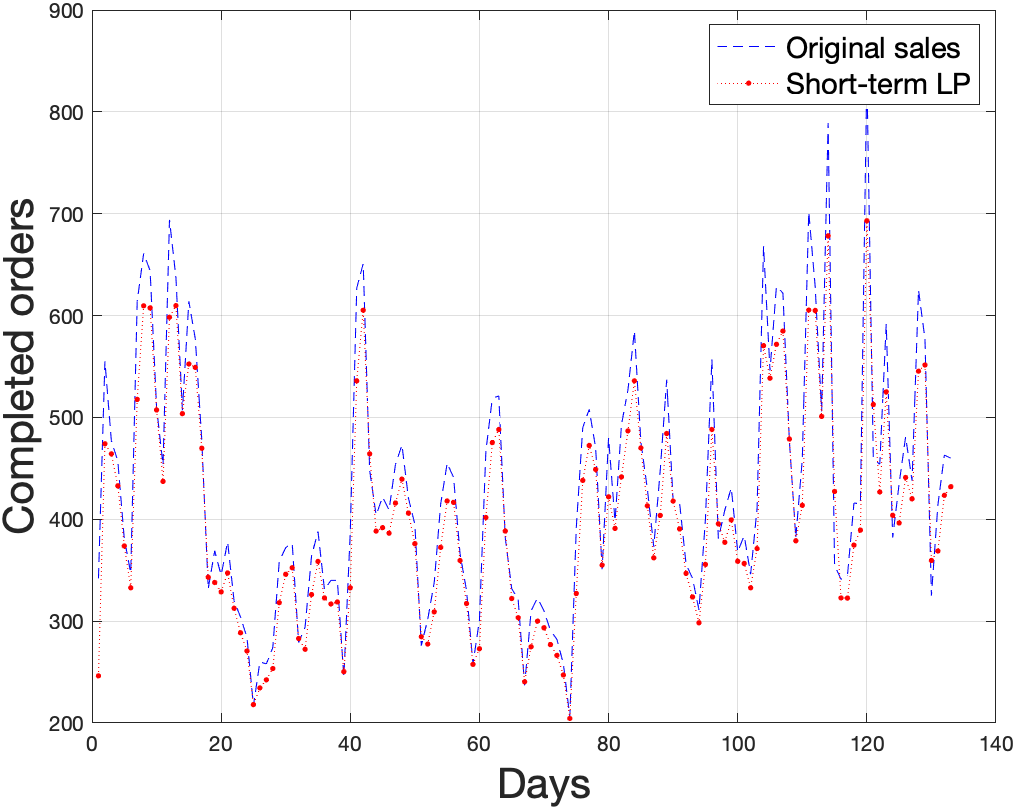
\includegraphics[width=1\textwidth]{figures/expLP.png}
                \caption{Results of short-term linear prediction.}
                \label{fig:slpres}
            \end{minipage}\hfill
            \begin{minipage}{0.45\textwidth}
                \centering
                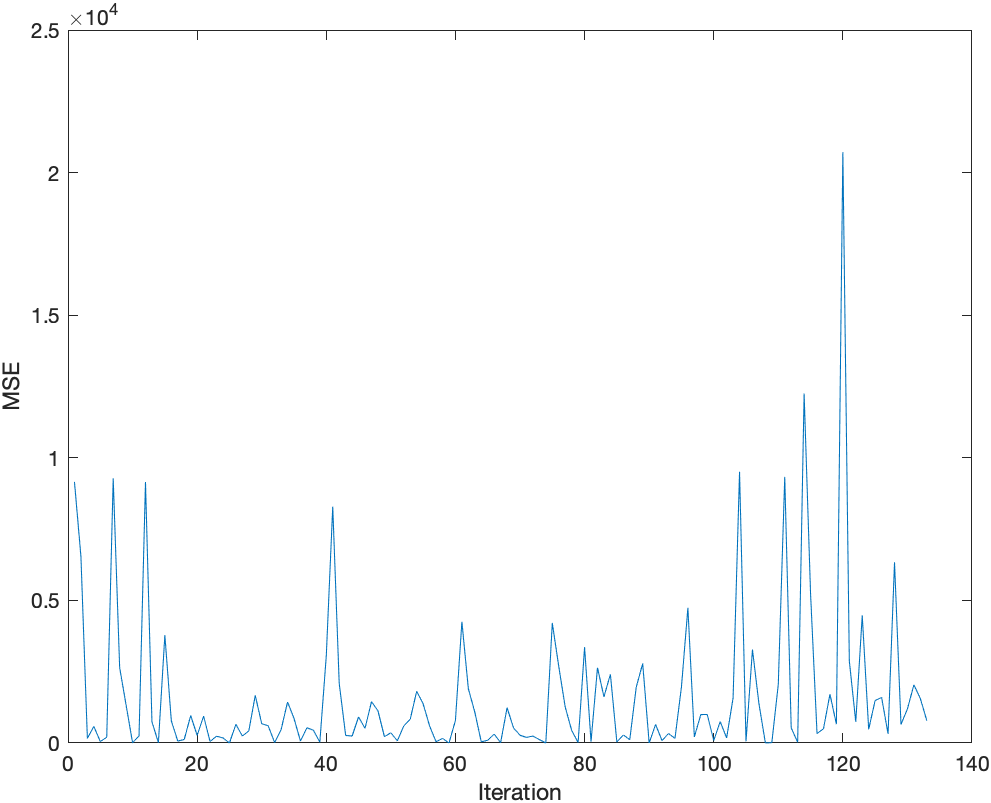
\includegraphics[width=\textwidth]{figures/expMseLP.png}
                \caption{MSE of short-term linear prediction.}
                \label{fig:slpmse}
            \end{minipage}
        \end{figure}
        \newpage
        \subsubsection{Extended short-term linear prediction} \label{subsec:res_estlp}
        After conducting our experiment, we calculated an R-squared (R2) value of 0.8881.
        This indicates that approximately 88.8\% of the variation in the dependent
        variable can be explained by the independent variables included in our model.\\
        \\
        We also determined that the root mean squared error (RMSE) is 40.4662.
        This means that, on average, there is a difference of approximately 40.4
        units between the predicted values from our model and the actual values.\\
        \\
        Additionally, we found that the mean squared error (MSE) is 1637.5.
        This suggests that, on average, the squared difference between the predicted
        and actual values is approximately 1650.1.
        \begin{figure}[h]
            \centering
            \begin{minipage}{0.45\textwidth}
                \centering
                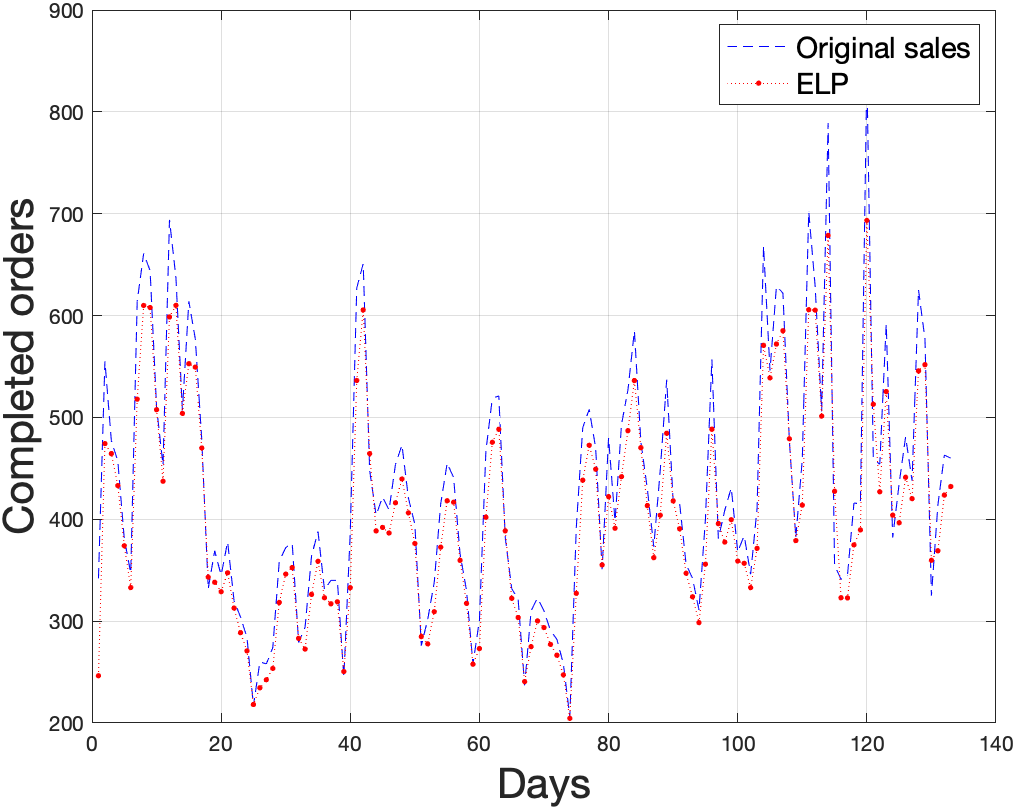
\includegraphics[width=1\textwidth]{figures/expELP.png}
                \caption{Results of extended short-term linear prediction.}
                \label{fig:eslpres}
            \end{minipage}\hfill
            \begin{minipage}{0.45\textwidth}
                \centering
                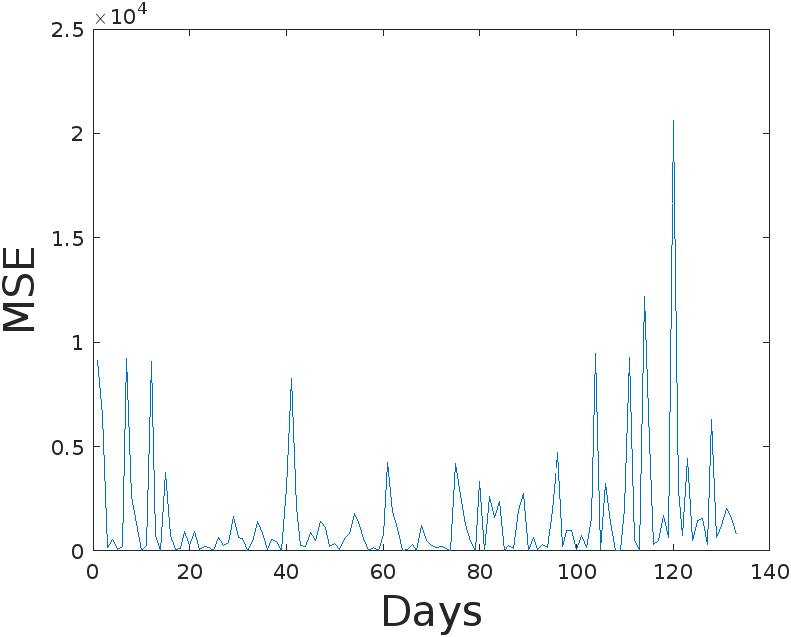
\includegraphics[width=1\textwidth]{figures/expMseELP.png}
                \caption{MSE of extended short-term linear prediction.}
                \label{fig:eslpmse}
            \end{minipage}
        \end{figure}

        \subsubsection{Long-term linear prediction} \label{subsec:res_ltlp}
        An R² value of 0.9160 means that 91.6\% of the variation in the dependent
        variable can be explained by the independent variables in the model.\\
        \\
        RMSE (Root Mean Square Error) and MSE (Mean Squared Error) are measures of the
        error or difference between the actual values of the dependent variable and the
        predicted values from the model. RMSE is the square root of the average squared
        difference between the predicted and actual values, while MSE is simply the
        average squared difference between them.\\
        \newpage
        In this case, an RMSE of 35.0163 means that on average, the predicted values from
        the model are about 35.02 units away from the actual values. And the
        MSE of 1223.3 means that on average, the squared difference between the predicted
        and actual values is 1223.3.
        \begin{figure}[h]
            \centering
            \begin{minipage}{0.45\textwidth}
                \centering
                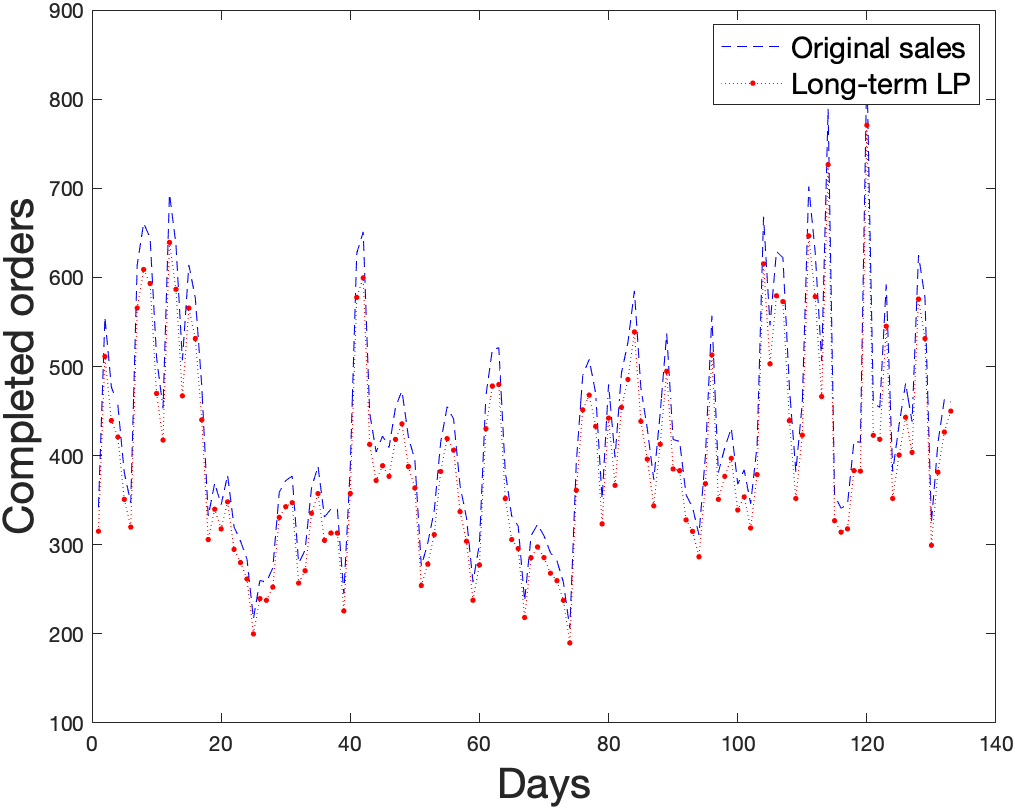
\includegraphics[width=1\textwidth]{figures/expLTLP.png}
                \caption{Results of long-term linear prediction.}
                \label{fig:ltlp}
            \end{minipage}\hfill
            \begin{minipage}{0.45\textwidth}
                \centering
                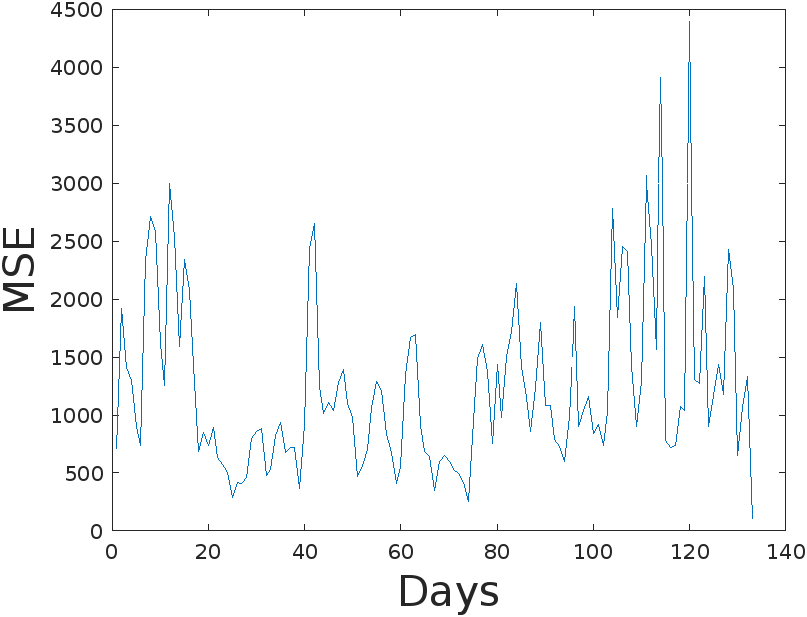
\includegraphics[width=1\textwidth]{figures/expMseLTLP.png}
                \caption{MSE of long-term linear prediction.}
                \label{fig:ltlpmse}
            \end{minipage}
        \end{figure}
        
        \subsubsection{Extended long-term linear prediction} \label{subsec:res_eltlp}
        The R-squared value of 0.9171 indicates that the independent variables in the
        model can explain about 91.7\% of the variation observed in the dependent variable.
        The RMSE and MSE are metrics used to evaluate the accuracy of the model's predictions
        compared to the actual values. The RMSE value of 34.7782 means that the average difference
        between the predicted and actual values is approximately 34.7 units. The MSE value of
        1206.7 indicates that the average squared difference between the predicted and actual
        values is approximately 1206.7.\\
        \begin{figure}[h]
            \centering
            \begin{minipage}{0.49\textwidth}
                \centering
                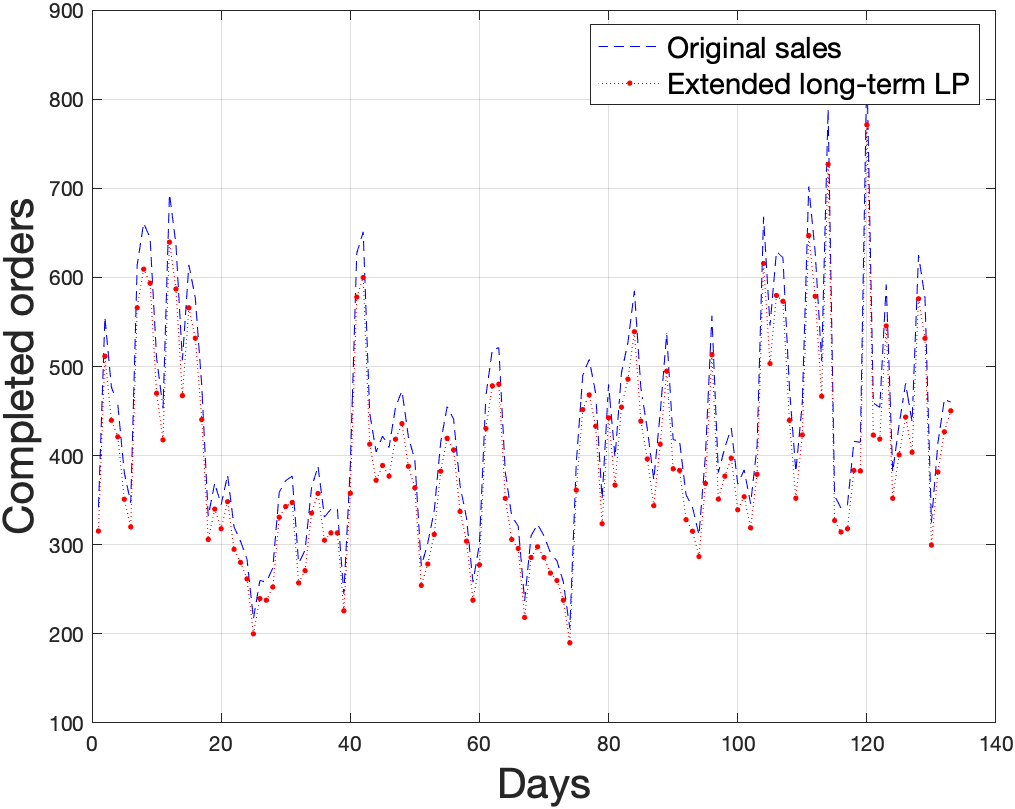
\includegraphics[width=0.8\textwidth]{figures/expELTLP.png}
                \caption{Results of extended long-term linear prediction.}
                \label{fig:eltlpres}
            \end{minipage}\hfill
            \begin{minipage}{0.49\textwidth}
                \centering
                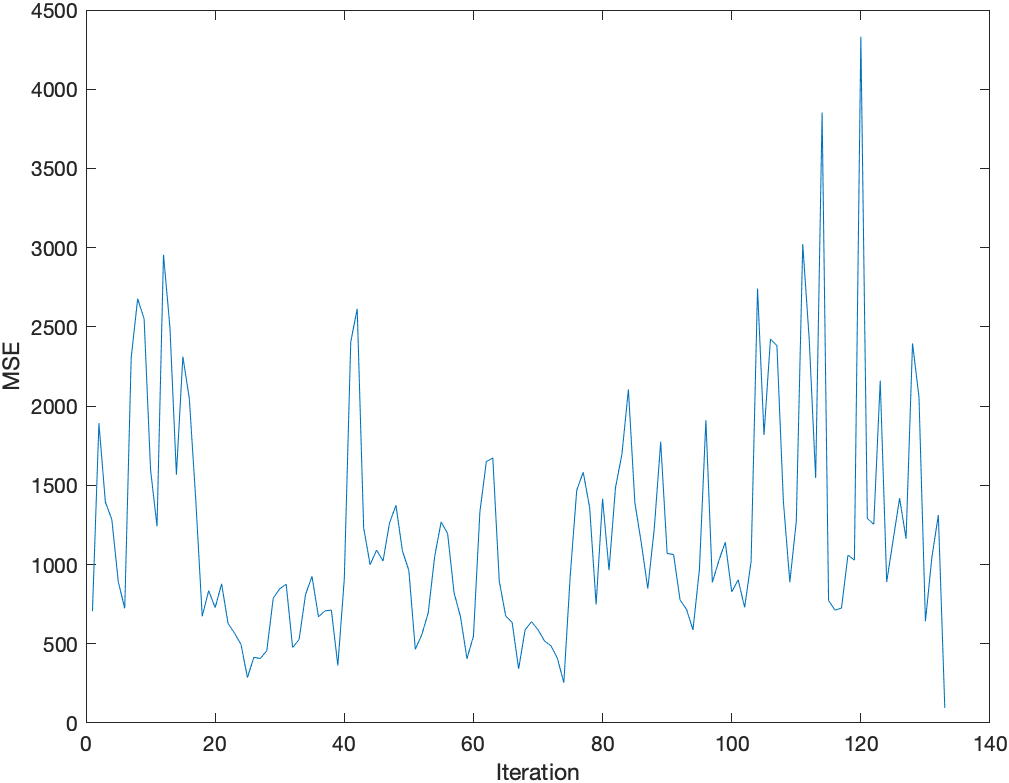
\includegraphics[width=0.8\textwidth]{figures/expMseELTLP.png}
                \caption{MSE of long-term linear prediction.}
                \label{fig:eltlpmse}
            \end{minipage}
        \end{figure}
        \newpage
        Overall, higher R-squared values and lower RMSE and MSE values in this model are
        desirable as they indicate a better fit of the model to the data and better predictive accuracy.
        \subsubsection{Comparison of the predictors} \label{subsec:res_comparison}
        Let's see results from our experiment in table \ref{tab:model_comparison} as we expected
        long term prediction is worst than long term prediction and apply extended weights to
        linear prediction made all comparison parameters better.\\
        \\
        On the figures with MSE representation we can see the main better point of long-term
        prediction for economical datasets. From $R^2$ and RMSE the improvments of the models is not
        see so higher than on the figures (\ref{fig:slpmse},\ref{fig:eslpmse},\ref{fig:ltlpmse}, \ref{fig:eltlpmse}).
        \begin{table}[!ht]
            \centering
            \begin{tabular}{|l|c|c|c|}
                \hline
                Model & $R^2$ & RMSE & MSE \\
                \hline
                Short-term linear prediction & 0.8872 & 40.6215 & 1650.1 \\
                Short-term extended linear prediction & 0.8881 & 40.4662 & 1637.5 \\
                Long-term linear prediction & 0.9160 & 35.0163 & 1223.3 \\
                Long-term extended linear prediction & 0.9171 & 34.7782 & 1206.7 \\
                \hline
            \end{tabular}
            \caption{Comparison of linear prediction models}
            \label{tab:model_comparison}
        \end{table}

        \begin{figure}[!ht]
            \begin{minipage}{0.45\textwidth}
                \centering
                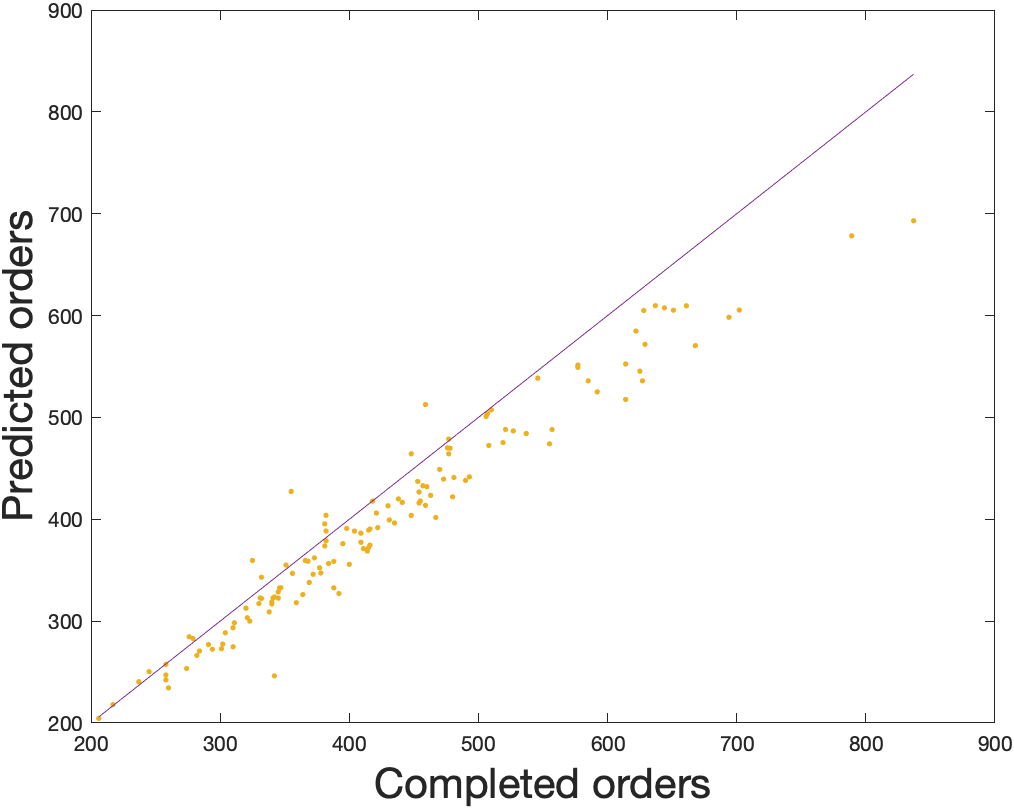
\includegraphics[width=1\textwidth]{figures/expCompLP.png}
                \caption{MSE success of prediction for short-term linear prediction.}
                \label{fig:stlpres}
            \end{minipage}\hfill
            \begin{minipage}{0.45\textwidth}
                \centering
                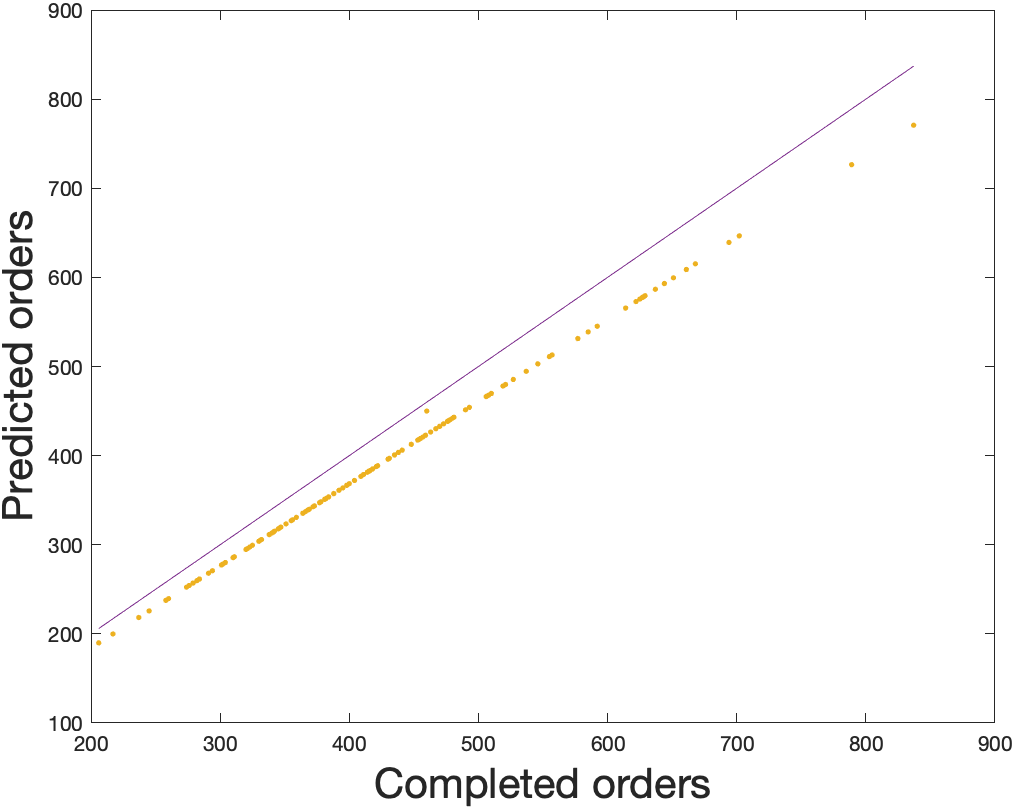
\includegraphics[width=1\textwidth]{figures/expCompLTLP.png}
                \caption{MSE success of prediction for long-term linear prediction.}
                \label{fig:eltlpres}
            \end{minipage}\hfill
        \end{figure}
        \newpage
        \begin{figure}[!ht]
            \centering
            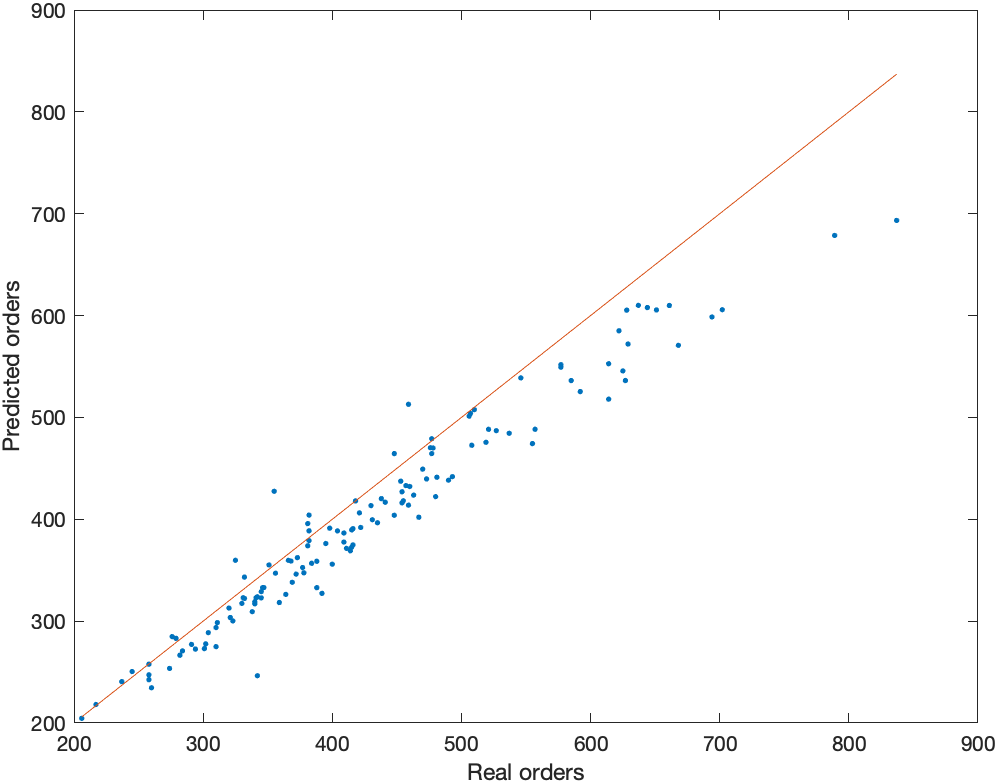
\includegraphics[width=0.8\textwidth]{figures/expCompELP.png}
            \caption{MSE success of prediction for extended short-term linear prediction.}
            \label{fig:eslpmse}
        \end{figure}
        \begin{figure}[!ht]
            \centering
            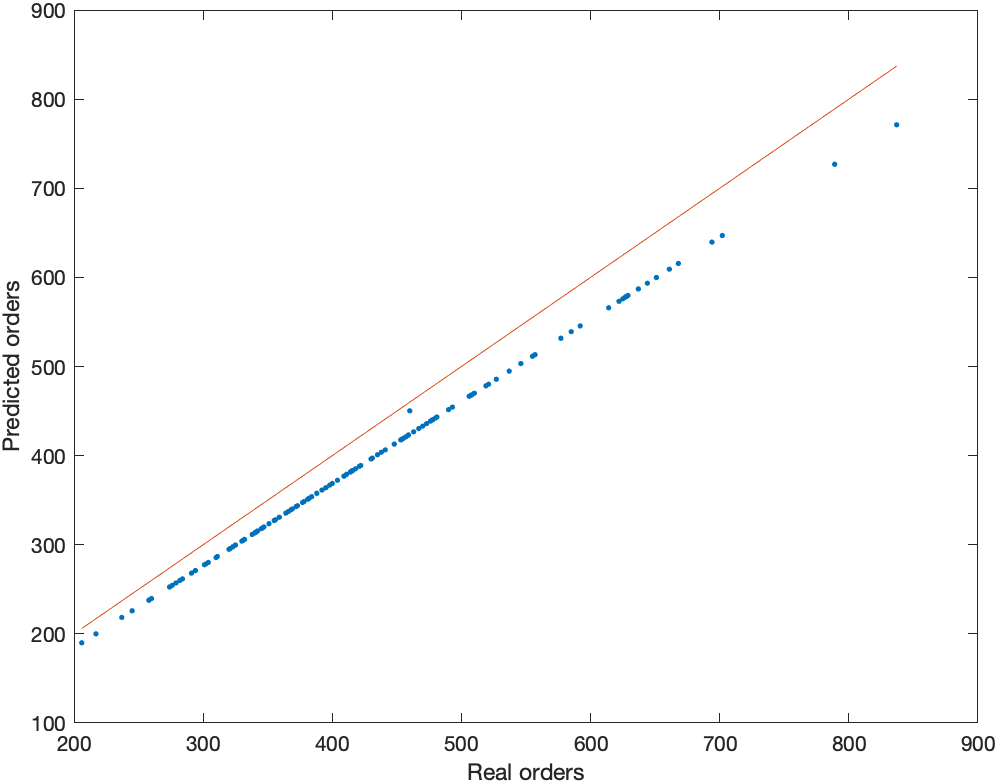
\includegraphics[width=0.8\textwidth]{figures/expCompELTLP.png}
            \caption{MSE success of prediction for long-term linear prediction.}
            \label{fig:eltlpmse}
        \end{figure}
